
\documentclass[spec, och, labwork]{shiza}
% параметр - тип обучения - одно из значений:
%    spec     - специальность
%    bachelor - бакалавриат (по умолчанию)
%    master   - магистратура
% параметр - форма обучения - одно из значений:
%    och   - очное (по умолчанию)
%    zaoch - заочное
% параметр - тип работы - одно из значений:
%    referat    - реферат
%    coursework - курсовая работа (по умолчанию)
%    diploma    - дипломная работа
%    pract      - отчет по практике
% параметр - включение шрифта
%    times    - включение шрифта Times New Roman (если установлен)
%               по умолчанию выключен
\usepackage{subfigure}
\usepackage{tikz,pgfplots}
\pgfplotsset{compat=1.5}
\usepackage{float}

%\usepackage{titlesec}
\setcounter{secnumdepth}{4}
%\titleformat{\paragraph}
%{\normalfont\normalsize}{\theparagraph}{1em}{}
%\titlespacing*{\paragraph}
%{35.5pt}{3.25ex plus 1ex minus .2ex}{1.5ex plus .2ex}

\titleformat{\paragraph}[block]
{\hspace{1.25cm}\normalfont}
{\theparagraph}{1ex}{}
\titlespacing{\paragraph}
{0cm}{2ex plus 1ex minus .2ex}{.4ex plus.2ex}

% --------------------------------------------------------------------------%


\usepackage[T2A]{fontenc}
\usepackage[utf8]{inputenc}
\usepackage{graphicx}
\graphicspath{ {./images/} }
\usepackage{tempora}

\usepackage[sort,compress]{cite}
\usepackage{amsmath}
\usepackage{amssymb}
\usepackage{amsthm}
\usepackage{fancyvrb}
\usepackage{listings}
\usepackage{listingsutf8}
\usepackage{longtable}
\usepackage{array}
\usepackage[final]{pdfpages}
\usepackage[english,russian]{babel}

% \usepackage[colorlinks=true]{hyperref}
\usepackage{url}

\usepackage{underscore}
\usepackage{setspace}
\usepackage{indentfirst} 
\usepackage{mathtools}
\usepackage{amsfonts}
\usepackage{enumitem}
\usepackage{tikz}

\newcommand{\eqdef}{\stackrel {\rm def}{=}}
\newcommand{\specialcell}[2][c]{%
\begin{tabular}[#1]{@{}c@{}}#2\end{tabular}}

\renewcommand\theFancyVerbLine{\small\arabic{FancyVerbLine}}

\newtheorem{lem}{Лемма}

\begin{document}

% Кафедра (в родительном падеже)
\chair{}

% Тема работы
\title{Теория псевдослучайных генераторов}

% Курс
\course{4}

% Группа
\group{431}

% Факультет (в родительном падеже) (по умолчанию "факультета КНиИТ")
\department{факультета КНиИТ}

% Специальность/направление код - наименование
%\napravlenie{09.03.04 "--- Программная инженерия}
%\napravlenie{010500 "--- Математическое обеспечение и администрирование информационных систем}
%\napravlenie{230100 "--- Информатика и вычислительная техника}
%\napravlenie{231000 "--- Программная инженерия}
\napravlenie{100501 "--- Компьютерная безопасность}

% Для студентки. Для работы студента следующая команда не нужна.
% \studenttitle{Студентки}

% Фамилия, имя, отчество в родительном падеже
\author{Ивнановой Ксении}

% Заведующий кафедрой
% \chtitle{} % степень, звание
% \chname{}

%Научный руководитель (для реферата преподаватель проверяющий работу)
\satitle{доцент} %должность, степень, звание
\saname{И. И. Слеповичев}

% Руководитель практики от организации (только для практики,
% для остальных типов работ не используется)
% \patitle{к.ф.-м.н.}
% \paname{С.~В.~Миронов}

% Семестр (только для практики, для остальных
% типов работ не используется)
%\term{8}

% Наименование практики (только для практики, для остальных
% типов работ не используется)
%\practtype{преддипломная}

% Продолжительность практики (количество недель) (только для практики,
% для остальных типов работ не используется)
%\duration{4}

% Даты начала и окончания практики (только для практики, для остальных
% типов работ не используется)
%\practStart{30.04.2019}
%\practFinish{27.05.2019}

% Год выполнения отчета
\date{2024}

\maketitle

% Включение нумерации рисунков, формул и таблиц по разделам
% (по умолчанию - нумерация сквозная)
% (допускается оба вида нумерации)
% \secNumbering

%-------------------------------------------------------------------------------------------
% \tableofcontents

  % -------------% -------------% -------------% -------------% -------------% -------------
  \section{Параметры и результаты запуска программы}

    \textbf{Линейный конгруэнтный метод}

    Параметры генерации:
 
  python3 main.py -g lc -i 1024,1664525,1013904223,1 -n 10000 -f lc.dat

  \vspace{5mm}
  % -------------% -------------% -------------% -------------% -------------% -------------
    \textbf{Аддитивный метод}

  Параметры генерации:

  python3 main.py -g add -i 30000,24,55,79,134,213,347,560,907,1467,2374,
  3841,6215,10056,16271,26327,12598,8925,21523,448,21971,22419,14390,6809,
  21199,28008,19207,17215,6422,23637,59,23696,23755,17451,11206,28657,9863,
  8520,18383,26903,15286,12189,27475,9664,7139,16803,23942,10745,4687,15432,
  20119,5551,25670,1221,26891,28112,23779,17506 -n 10000 -f add.dat
  \vspace{5mm}
 
% -------------% -------------% -------------% -------------% -------------% -------------
    \textbf{Пятипараметрический метод}

  Параметры генерации:
 
  python3 main.py -g 5p -i 89,7,13,24,10,234122131 -n 10000 -f 5p.dat
  \vspace{5mm}
% -------------% -------------% -------------% -------------% -------------% -------------

    \textbf{Регистр сдвига с обратной связью (РСЛОС)}

    Параметры генерации:
 
  python3 main.py -g lfsr -i 10011011010011010,000101000111 -n 10000 -f lfsr.dat
  \vspace{5mm}

  % -------------% -------------% -------------% -------------% -------------% -------------

    \textbf{Нелинейная комбинация РСЛОС}

    Параметры генерации:

  python3 main.py -g nfsr -i 00000001010101,01011100000111101,\\
  010101001100000,0001001,10000010010,000000001,1001 -f nfsr.dat 
  -n 10000
  \vspace{5mm}
 % -------------% -------------% -------------% -------------% -------------% -------------

 \textbf{Вихрь Мерсенна}

 Параметры генерации:
 
  python3 main.py -g mt -i 1000,1234 -n 10000 -f mt.dat
  \vspace{5mm}
% -------------% -------------% -------------% -------------% -------------% -------------
 \textbf{RC4}

  Параметры генерации:
 
  python3 main.py -g rc4 -i 213,968,838,64,355,214,212,36,695,139,897518,656,\\
  956,810,510,985,105,670,8,907,951,685,989,222,931,169,286,289,556,731,902,\\
  688,701,771,533,990,630,708,884,255,683,25,214,792,348,34,758,9,781,946,\\
  580,615,955,585,5,886,563,81,38,809,444,619,222,544,53,635,621,630,251,497,\\
  257,2,467,897,790,728,676,722,838,465,781,10,828,903,235,857,841,146,719,\\
  681,678,961,652,491,38,256,909,251,21,110,811,273,25,642,286,489,478,184,812,\\
  770,846,241,141,266,500,375,827,633,761,154,663,461,206,529,212,667,342,360,\\
  165,523,749,582,803,553,345,786,990,361,702,256,380,234,238,73,965,266,300,\\
  847,755,969,681,146,843,125,306,845,752,879,458,788,833,727,817,122,239,765,\\
  877,827,327,733,658,644,880,150,474,493,689,670,368,611,263,113,417,834,103,\\
  725,754,117,824,623,338,540,337,879,521,183,370,808,120,571,871,301,210,796,\\
  744,398,106,845,745,842,876,399,27,105,601,802,831,53,266,157,352,175,303,\\
  505,484,994,425,292,729,654,584,860,420,412,49,281,417,703,400,48,404,772,\\389,
  733,152,271,585,404,333,381,696,928,609,659,180,10 -f rc.dat -n 10000
  \vspace{5mm}

  % -------------% -------------% -------------% -------------% -------------% -------------
 \textbf{ГПСЧ на основе RSA}

 Параметры генерации:

  python3 main.py -g rsa -i 10967,571,77,10 -n 10000 -f rsa.dat
 \vspace{5mm}

% -------------% -------------% -------------% -------------% -------------% -------------
 \textbf{Алгоритм Блюм-Блюма-Шуба}

  Параметры генерации:
 
  python3 main.py -g bbs -i 15621,10 -n 10000 -f bbs.dat

  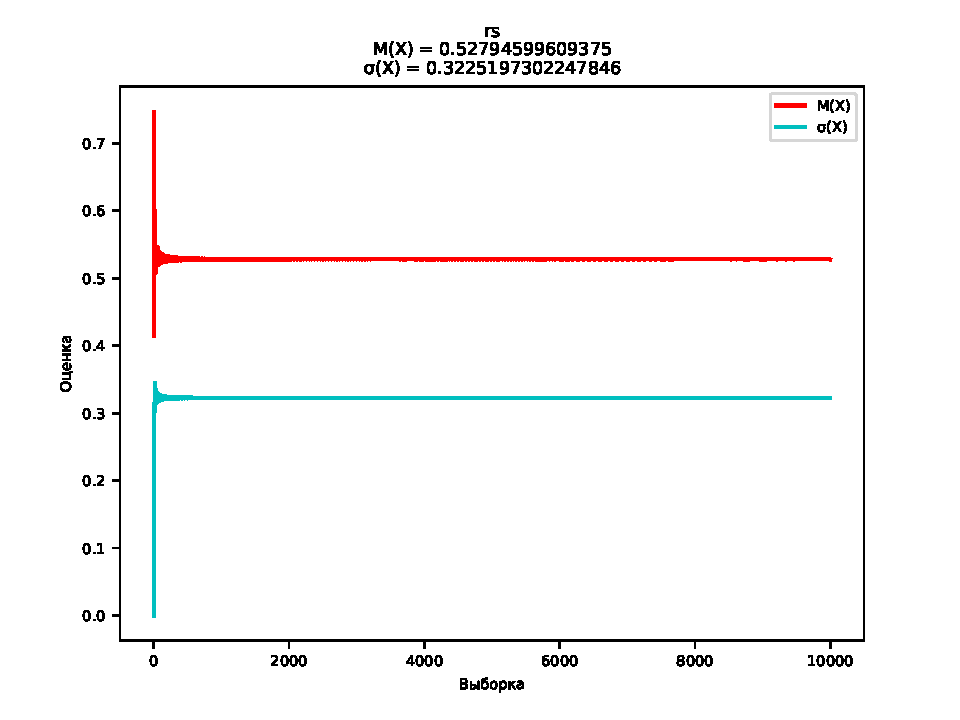
\includepdf[pages=-,pagecommand={},width=\textwidth]{allplots.pdf}
  % \includepdf[pages=1-6]{all_plots.pdf}

\subsection{Оценки параметров ППСЧ}
\begin{flushleft}
  \centering
  \begin{tabular}[t]{|p{1cm}|p{5cm}|p{5cm}|} \hline 
      	  & $M(X)$ & $\sigma (X)$ \\[2mm]\hline
    lc	  & 0.5001070313       &  0.2885282436     \\[2mm]\hline
    add   & 0.4959591797	     &  0.2872104607    \\[2mm]\hline
    5p    & 0.5076768555	     &  0.2892557885    \\[2mm]\hline
    lfsr  & 0.5003677734	     &  0.2893232094    \\[2mm]\hline
    nfsr  & 0.4995135742	     &  0.2888325181    \\[2mm]\hline
    mt    & 0.488571875	       &  0.2811702731    \\[2mm]\hline
    rc4   & 0.4899671875	     &  0.2894136027    \\[2mm]\hline
    rsa   & 0.5279459961	     &  0.3225197302    \\[2mm]\hline
    bbs   & 0.388540918	       &  0.2828818654    \\[2mm]\hline
  
\end{tabular}
\end{flushleft}

\subsection{Проверка последовательностей на тестах }
\begin{flushleft}
    \begin{tabular}[t]{|p{3cm}|p{1cm}|p{1cm}|p{1cm}|p{1cm}|p{1cm}|p{1cm}|p{1cm}|p{1cm}|p{1cm}|} \hline 
                  & lc	&  add	&  5p	& lfsr	& nfsr  & mt	& rc4	& rsa	& bbs \\[2mm]\hline
    Хи-квадрат	  &  +  &   +   &  +  &  +    & 	-   &  -  &  -  &  -  &  -  \\[2mm]\hline
    серий	        &  -  &   +   &  -  &  -    &   -   &  -  &  -	&  -  &  +  \\[2mm]\hline
    интервалов  	&  +  &   -   &  +  &  +    &   +   &  +  &  +  &  +  &  -  \\[2mm]\hline
    разбиений	    &  -  &   +   &  -	&  -    &   -   &  -  &  -  &  -  &  -  \\[2mm]\hline
    перестановок	&  -  &   +   &  -	& -     &   -   &  -  &  -  &  -  &  -  \\[2mm]\hline
    монотонности	&  -  &   +   &  -	& -     &   -   &  -  &  -  &  -  &  -  \\[2mm]\hline
    % конфликтов	  &    &  	    &  	  & 	    & 	    & 	  & 	  &     &     \\[2mm]\hline
  \end{tabular}
\end{flushleft}
\end{document}
